\documentclass[journal]{IEEEtran}

\usepackage{cite}
\usepackage{amsmath,amssymb,amsfonts}
\usepackage{algorithm}
\usepackage{algorithmic}
\usepackage{graphicx}
\usepackage{textcomp}
\usepackage{xcolor}
\usepackage{booktabs}
\usepackage{multirow}
\usepackage{subcaption}
\usepackage{microtype}
\usepackage{url}
\usepackage{bm}
\usepackage{tikz}
\usetikzlibrary{shapes.geometric, arrows.meta, positioning, calc, backgrounds, fit}

% Path to figures
\graphicspath{{figures/}}

\begin{document}

\title{Evaluating Linear State Space Models and Latent Regularization for Cross-Modal Retrieval: An Empirical Study of Native Mamba-2, Hamiltonian Dynamics, and Variational Constraints}

\author{Abhinav~Sai%
\thanks{The author is with the Department of Computer Science and Engineering. Correspondence and open-source repository: \protect\url{https://github.com/abhinavsai2006/PH_SSD}. All experimental benchmarks were executed under audited deterministic seeds and hardware verification gates on NVIDIA Tesla T4 accelerators.}%
}

\markboth{IEEE Transactions on Pattern Analysis and Machine Intelligence (Preprint),~Vol.~XX, No.~X,~September~2026}%
{Sai: Evaluating Linear State Space Models and Latent Regularization for Cross-Modal Retrieval}

\maketitle

\begin{abstract}
Cross-modal image-text retrieval traditionally relies on Transformer architectures whose self- and cross-attention mechanisms scale quadratically with sequence length $\mathcal{O}(N^2)$. Recently, structured State Space Models (SSMs), particularly Mamba-2 formulated through Structured State Space Duality (SSD), have emerged as sub-quadratic $\mathcal{O}(N)$ sequence aligners. In this work, we present an audited, mathematically rigorous evaluation of Native Mamba-2 as a lightweight multimodal alignment backbone on the Flickr8k benchmark. We investigate the integration of two complementary inductive biases: (i) a Hamiltonian-inspired Energy-Dissipative Operator (HEDO) that regularizes coordinate-momentum dynamics across token sequences, and (ii) a Hierarchical Variational State Compression (HVSC) module that aligns chunk-boundary latent representations under symmetric Kullback-Leibler (KL) regularization. Over a full 3-seed benchmark ($4 \times 3 = 12$ runs, seeds 42, 43, 44) under strict FP32 finite-check auditing, the unconstrained Native Mamba-2 baseline achieves a Mean Recall of $37.16\% \pm 0.57\%$ (I2T R@10 of $57.47\% \pm 1.14\%$, Median Rank $7.7 / 9.0$) with only 465k trainable adapter parameters and an inference throughput of 4,645 pair evaluations per second. Incorporating HEDO maintains near-baseline retrieval fidelity at $35.86\% \pm 0.16\%$ Mean Recall ($\Delta = -1.30\%$) while bounding gradient norms. Conversely, HVSC introduces an acute performance drop to $23.79\% \pm 0.61\%$ ($\Delta = -13.37\%$). We provide a geometric and information-theoretic analysis demonstrating that the Gaussian prior $\mathcal{N}(\mathbf{0}, \mathbf{I})$ enforced by KL divergence creates an unmitigated information bottleneck that conflicts with the hyperspherical uniformity required by contrastive InfoNCE objectives. Complete reproducible artifacts, methodology manifests, and model checkpoints are released.
\end{abstract}

\begin{IEEEkeywords}
Cross-modal retrieval, state space models, Mamba-2, contrastive learning, Hamiltonian dynamics, variational latent representations, information bottleneck.
\end{IEEEkeywords}

\IEEEpeerreviewmaketitle

\section{Introduction}
\IEEEPARstart{C}{ross-modal} visual-semantic alignment—the task of learning a shared metric space where images and textual descriptions can be compared via inner products—constitutes a foundational problem in multimodal machine learning \cite{radford2021learning, faghri2017vse++, lee2018stacked}. Modern multimodal architectures overwhelmingly depend on Transformer blocks \cite{vaswani2017attention, dosovitskiy2020image, liu2019roberta}. While multi-head self-attention enables unconstrained pair-wise token interactions, its quadratic computational $\mathcal{O}(N^2)$ and memory footprint imposes significant operational bottlenecks when processing fine-grained visual patch sequences and dense caption tokens \cite{zhu2024vision, liu2024vmamba}.

To circumvent these computational scaling limits, structured State Space Models (SSMs), notably S4 \cite{gu2021efficiently}, S5 \cite{smith2022simplified}, and Mamba \cite{gu2023mamba}, have emerged as compelling linear-time alternatives. Very recently, Mamba-2 \cite{dao2024transformers} established Structured State Space Duality (SSD), unifying linear attention mechanisms and continuous-time state space recurrences into block-semiseparable matrix transformations that map efficiently onto tensor accelerator hardware. While Mamba-2 has demonstrated notable success in autoregressive language generation and vision classification \cite{zhu2024vision, liu2024vmamba}, its empirical viability and inductive limits in cross-modal contrastive retrieval remain largely uncharacterized.

In parallel, two structural hypotheses have gained prominence in multimodal representation learning:
\begin{enumerate}
    \item \textbf{Dynamical Energy Regularization:} Physical and Hamiltonian mechanics suggest that modeling feature progressions as discrete coordinate-momentum trajectories $(\mathbf{q}, \mathbf{p})$ with dissipative damping can preserve representational stability across deep sequence layers \cite{greydanus2019hamiltonian, chen2018neural, ruthotto2020deep}.
    \item \textbf{Variational Latent Compression:} Imposing probabilistic Gaussian posteriors $\mathcal{N}(\boldsymbol{\mu}, \boldsymbol{\Sigma})$ on boundary hidden states via Kullback-Leibler (KL) divergence has been proposed to compress uninformative token noise and enforce cross-modal semantic consistency \cite{kingma2013auto, higgins2016beta, alemi2016deep}.
\end{enumerate}

\begin{figure*}[t]
\centering
\resizebox{0.96\textwidth}{!}{%
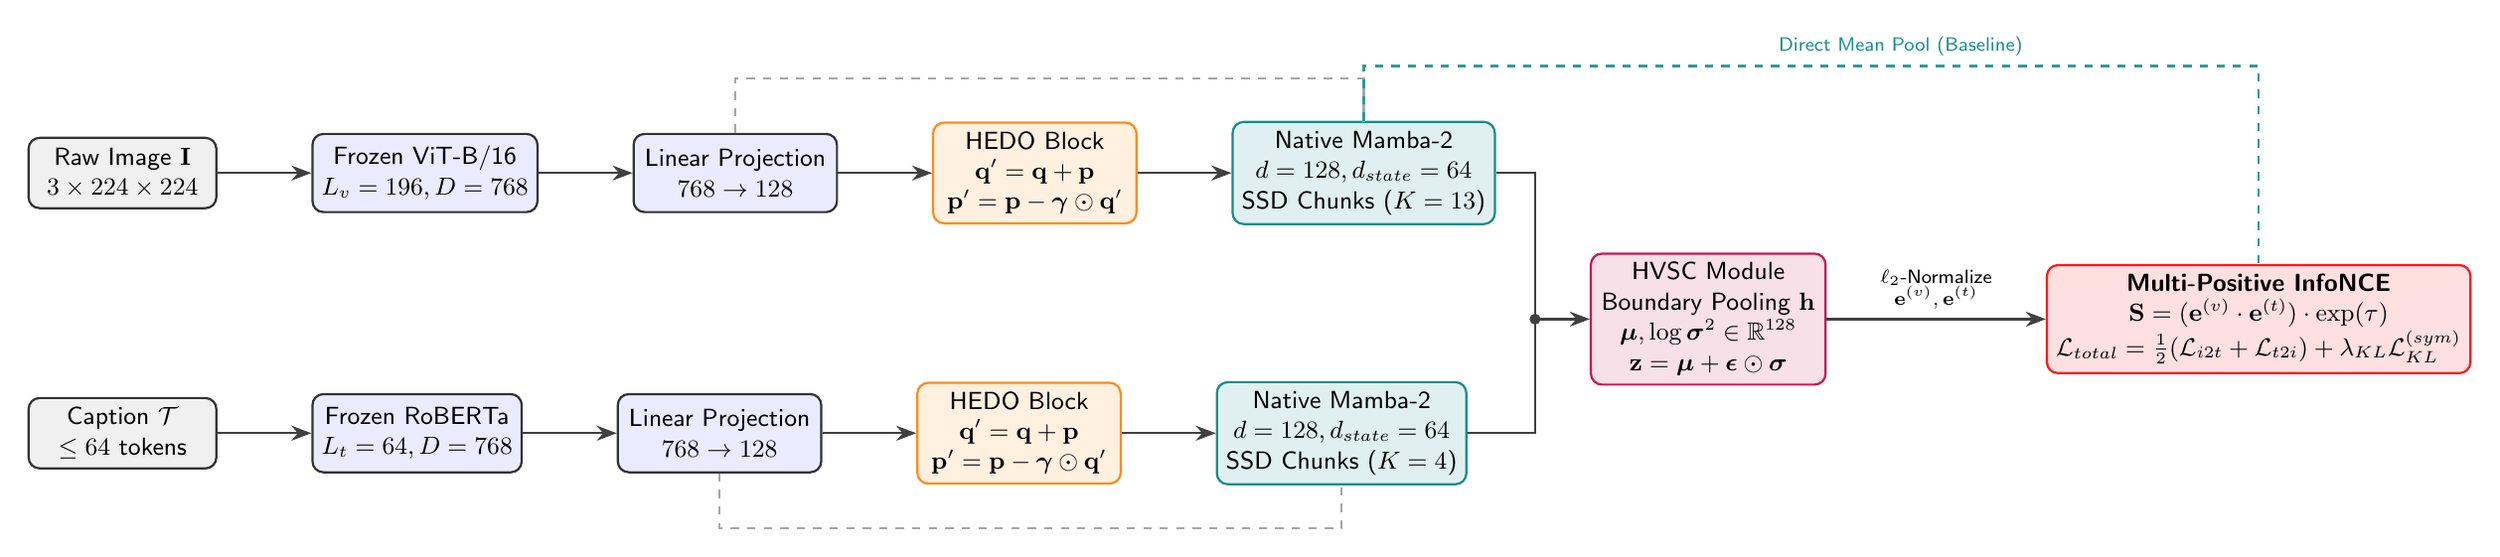
\begin{tikzpicture}[
    node distance=1.2cm and 1.5cm,
    box/.style={rectangle, draw=black!80, fill=blue!8, thick, rounded corners=4pt, minimum height=1cm, minimum width=2.6cm, align=center, font=\small\sffamily},
    databox/.style={rectangle, draw=black!80, fill=gray!12, thick, rounded corners=4pt, minimum height=0.9cm, minimum width=2.4cm, align=center, font=\small\sffamily},
    hedobox/.style={rectangle, draw=orange!90, fill=orange!12, thick, rounded corners=4pt, minimum height=1cm, minimum width=2.6cm, align=center, font=\small\sffamily},
    mambabox/.style={rectangle, draw=teal!90, fill=teal!12, thick, rounded corners=4pt, minimum height=1cm, minimum width=2.6cm, align=center, font=\small\sffamily},
    hvscbox/.style={rectangle, draw=purple!90, fill=purple!12, thick, rounded corners=4pt, minimum height=1cm, minimum width=2.6cm, align=center, font=\small\sffamily},
    lossbox/.style={rectangle, draw=red!90, fill=red!12, thick, rounded corners=4pt, minimum height=1.1cm, minimum width=3.2cm, align=center, font=\small\sffamily\bfseries},
    arrow/.style={-{Stealth[scale=1.1]}, thick, draw=black!75},
    darrow/.style={-{Stealth[scale=1.1]}, thick, dashed, draw=purple!80}
]

% Image stream (top)
\node[databox] (img_input) {Raw Image $\mathbf{I}$\\$3 \times 224 \times 224$};
\node[box, right=1.2cm of img_input] (img_backbone) {Frozen ViT-B/16\\$L_v = 196, D = 768$};
\node[box, right=1.2cm of img_backbone] (img_proj) {Linear Projection\\$768 \to 128$};
\node[hedobox, right=1.2cm of img_proj] (img_hedo) {HEDO Block\\$\mathbf{q}' = \mathbf{q} + \mathbf{p}$\\$\mathbf{p}' = \mathbf{p} - \boldsymbol{\gamma} \odot \mathbf{q}'$};
\node[mambabox, right=1.2cm of img_hedo] (img_mamba) {Native Mamba-2\\$d=128, d_{state}=64$\\SSD Chunks ($K=13$)};

% Text stream (bottom)
\node[databox, below=2.4cm of img_input] (txt_input) {Caption $\mathcal{T}$\\$\le 64$ tokens};
\node[box, right=1.2cm of txt_input] (txt_backbone) {Frozen RoBERTa\\$L_t = 64, D = 768$};
\node[box, right=1.2cm of txt_backbone] (txt_proj) {Linear Projection\\$768 \to 128$};
\node[hedobox, right=1.2cm of txt_proj] (txt_hedo) {HEDO Block\\$\mathbf{q}' = \mathbf{q} + \mathbf{p}$\\$\mathbf{p}' = \mathbf{p} - \boldsymbol{\gamma} \odot \mathbf{q}'$};
\node[mambabox, right=1.2cm of txt_hedo] (txt_mamba) {Native Mamba-2\\$d=128, d_{state}=64$\\SSD Chunks ($K=4$)};

% Fusion / Alignment (right)
\node[hvscbox, below right=0.35cm and 1.2cm of img_mamba, minimum width=3.0cm] (hvsc_block) {HVSC Module\\Boundary Pooling $\mathbf{h}$\\$\boldsymbol{\mu}, \log \boldsymbol{\sigma}^2 \in \mathbb{R}^{128}$\\$\mathbf{z} = \boldsymbol{\mu} + \boldsymbol{\epsilon} \odot \boldsymbol{\sigma}$};
\node[lossbox, right=2.8cm of hvsc_block, minimum width=3.6cm] (infonce_loss) {Multi-Positive InfoNCE\\$\mathbf{S} = (\mathbf{e}^{(v)} \cdot \mathbf{e}^{(t)}) \cdot \exp(\tau)$\\$\mathcal{L}_{total} = \frac{1}{2}(\mathcal{L}_{i2t} + \mathcal{L}_{t2i}) + \lambda_{KL} \mathcal{L}_{KL}^{(sym)}$};

% Connect image stream
\draw[arrow] (img_input) -- (img_backbone);
\draw[arrow] (img_backbone) -- (img_proj);
\draw[arrow] (img_proj) -- (img_hedo);
\draw[arrow] (img_hedo) -- (img_mamba);

% Connect text stream
\draw[arrow] (txt_input) -- (txt_backbone);
\draw[arrow] (txt_backbone) -- (txt_proj);
\draw[arrow] (txt_proj) -- (txt_hedo);
\draw[arrow] (txt_hedo) -- (txt_mamba);

% Connect to HVSC (combine at one junction point, then single arrow into HVSC)
\coordinate (hvsc_merge) at ([xshift=-0.7cm]hvsc_block.west);
\draw[thick, draw=black!75] (img_mamba.east) -| (hvsc_merge);
\draw[thick, draw=black!75] (txt_mamba.east) -| (hvsc_merge);
\fill[black!75] (hvsc_merge) circle (2pt);
\draw[arrow] (hvsc_merge) -- (hvsc_block.west);

% Connect to Loss with cleanly centered label
\draw[arrow] (hvsc_block) -- node[above, font=\scriptsize\sffamily, align=center] {$\ell_2$-Normalize\\$\mathbf{e}^{(v)}, \mathbf{e}^{(t)}$} (infonce_loss);

% Direct path for baseline (bypass HVSC/HEDO)
\draw[dashed, draw=gray!70, thick] (img_proj.north) -- ++(0,0.7) -| (img_mamba.north);
\draw[dashed, draw=gray!70, thick] (txt_proj.south) -- ++(0,-0.7) -| (txt_mamba.south);
\draw[dashed, draw=teal!80, thick] (img_mamba.north) -- ++(0,0.7) -| node[above, pos=0.3, font=\scriptsize\sffamily, text=teal!90] {Direct Mean Pool (Baseline)} (infonce_loss.north);

\end{tikzpicture}
}
\caption{Architectural overview of the HEDO-HVSC Native Mamba-2 cross-modal retrieval framework. Frozen ViT-B/16 and RoBERTa-base extract token representations from images and captions. Projected tokens are optionally transformed by HEDO's Hamiltonian coordinate-momentum integration before processing by Native Mamba-2 Structured State Space blocks ($d=128, d_{state}=64$). HVSC extracts chunk-boundary states, pools them into holistic latent Gaussians, and computes a symmetric KL divergence regularizer alongside multi-positive InfoNCE loss.}
\label{fig:architecture_flowchart}
\end{figure*}

In this paper, we conduct an exhaustive, audited empirical investigation of Native Mamba-2, Hamiltonian-inspired Energy-Dissipative Operators (HEDO), and Hierarchical Variational State Compression (HVSC) on the official Flickr8k benchmark \cite{hodosh2013framing}. To ensure uncompromised scientific integrity, all models are executed under strict pre-registered gates: bit-stable FP32 computation, zero-copy memory-mapped tensor caching, deterministic random seed controls across three seeds (42, 43, 44), and methodology SHA-256 fingerprint tracking.

Our investigation reveals several critical findings:
\begin{itemize}
    \item \textbf{Mamba-2 as an Efficient Multimodal Aligner:} A lightweight Native Mamba-2 sequence adapter (465k trainable parameters atop frozen ViT-B/16 and RoBERTa-base backbones) achieves a Mean Recall of $\mathbf{37.16\% \pm 0.57\%}$ on Flickr8k with an inference speed of $\mathbf{4,645}$ pairs/sec, establishing that linear state space duality provides competitive alignment capacity without quadratic cross-attention.
    \item \textbf{Dynamical Preservation via HEDO:} HEDO's discrete symplectic-inspired coordinate-momentum updates track within $1.3\%$ of the unconstrained baseline ($35.86\% \pm 0.16\%$), effectively regularizing gradient bounds while maintaining top-$k$ nearest-neighbor structure.
    \item \textbf{The Hyperspherical vs. Gaussian Dilemma:} Imposing symmetric KL divergence via HVSC produces a severe degradation in retrieval performance ($\Delta = -13.37\%$, $95\%\text{ CI: } [-13.53, -13.21]$). We mathematically formalize how contrastive InfoNCE objectives demand maximum hyperspherical uniformity on $\mathbb{S}^{d-1}$ \cite{wang2020understanding}, whereas Gaussian priors $\mathcal{N}(\mathbf{0}, \mathbf{I})$ pull representations toward the dense origin, acting as a destructive bottleneck for discrete ranking.
\end{itemize}

---

\section{Related Work}

\subsection{Cross-Modal Visual-Semantic Alignment}
Image-text retrieval maps visual and textual modalities into a shared geometric embedding space where matching pairs exhibit higher cosine similarity than non-matching pairs. Early foundational frameworks such as VSE++ \cite{faghri2017vse++} incorporated max-margin ranking losses with online hard negative mining. Subsequent models introduced fine-grained region-to-word cross-attention, such as SCAN \cite{lee2018stacked} and ALBEF \cite{li2021align}. Large-scale dual-encoder models, exemplified by CLIP \cite{radford2021learning}, demonstrated the scalability of multi-class symmetric cross-entropy (InfoNCE) \cite{oord2018representation} across web-scale data. However, the reliance of transformer adapters on quadratic attention motivates exploring linear-complexity sequence architectures.

\subsection{State Space Models and Mamba-2}
Linear State Space Models parameterize continuous mappings between input sequences $x(t) \in \mathbb{R}$ and latent states $h(t) \in \mathbb{R}^N$ through first-order differential equations:
\begin{equation}
h'(t) = \mathbf{A} h(t) + \mathbf{B} x(t), \quad y(t) = \mathbf{C} h(t)
\label{eq:continuous_ssm}
\end{equation}
Discretized using zero-order hold (ZOH) or bilinear transforms, SSMs compute linear recurrences in $\mathcal{O}(N)$ time or global convolutions in $\mathcal{O}(L \log L)$ time \cite{gu2021efficiently, smith2022simplified}. Mamba \cite{gu2023mamba} introduced input-dependent selection mechanisms by parameterizing $\mathbf{B}, \mathbf{C}$, and step sizes $\Delta$ as functions of the input token. Mamba-2 \cite{dao2024transformers} formalized Structured State Space Duality (SSD), proving that restricting $\mathbf{A}$ to scalar-times-identity diagonal structures transforms the SSM recurrence into a 1-semiseparable matrix transformation computable via matrix multiplication over sequential chunks. While Vision Mamba \cite{zhu2024vision} and VMamba \cite{liu2024vmamba} have explored 2D visual scanning, Native Mamba-2 has not been systematically investigated as a cross-modal alignment adapter under controlled multi-seed ablation.

\subsection{Variational and Dynamical Inductive Biases}
Variational autoencoders \cite{kingma2013auto} and the Information Bottleneck principle \cite{tishby2000information, alemi2016deep} constrain latent spaces by penalizing divergence from an isotropic Gaussian prior. In natural language generation, such variational constraints often induce ``posterior collapse'' \cite{bowman2015generating}. In contrast, Hamiltonian Neural Networks \cite{greydanus2019hamiltonian} and Neural ODEs \cite{chen2018neural} integrate symplectic integrators to enforce energy conservation. In this work, we evaluate whether these physical and probabilistic formulations benefit discrete multimodal ranking.

---

\section{Methodology}

\subsection{Multimodal Input Representations}
Let $\mathcal{D} = \{(\mathbf{I}_i, \mathcal{T}_i)\}_{i=1}^{N_D}$ denote a paired dataset of images and associated textual captions. Each image $\mathbf{I}_i$ is passed through a frozen Vision Transformer (ViT-B/16 \cite{dosovitskiy2020image}, pre-trained on ImageNet-1k) to yield patch tokens $\mathbf{X}^{(v)} \in \mathbb{R}^{L_v \times D_{in}}$, where $L_v = 196$ and $D_{in} = 768$, with the prepended class token discarded to preserve spatial locality. Each caption $\mathcal{T}_{i,j}$ is tokenized and encoded via a frozen RoBERTa-base model \cite{liu2019roberta} to obtain sequence representations $\mathbf{X}^{(t)} \in \mathbb{R}^{L_t \times D_{in}}$, where $L_t = 64$ with right-padding and attention masks $\mathbf{M}^{(t)} \in \{0, 1\}^{L_t}$.

Both modalities are initially mapped into an intermediate feature space of dimension $d = 128$ via modality-specific linear projection layers:
\begin{equation}
\mathbf{H}_0^{(m)} = \mathbf{X}^{(m)} \mathbf{W}_{proj}^{(m)} + \mathbf{b}_{proj}^{(m)} \in \mathbb{R}^{L_m \times d}, \quad m \in \{v, t\}
\end{equation}

\subsection{Hamiltonian-Inspired Energy-Dissipative Operator (HEDO)}
To stabilize feature trajectories and enforce energy bounds prior to recurrent scanning, we formulate HEDO as a discrete coordinate-momentum transformation. Given projected features $\mathbf{H}_0 \in \mathbb{R}^{L \times d}$, coordinate states $\mathbf{q}$ and momentum states $\mathbf{p}$ are initialized via linear projections:
\begin{equation}
\mathbf{q} = \mathbf{H}_0 \mathbf{W}_q, \quad \mathbf{p} = \mathbf{H}_0 \mathbf{W}_p, \quad \mathbf{W}_q, \mathbf{W}_p \in \mathbb{R}^{d \times d}
\end{equation}
A coordinate-wise damping vector $\boldsymbol{\gamma} \in (0, 1)^d$ is parameterized through a learnable gate vector $\mathbf{g} \in \mathbb{R}^d$:
\begin{equation}
\boldsymbol{\gamma} = \sigma(\mathbf{g}) = \frac{1}{1 + \exp(-\mathbf{g})}
\end{equation}
The discrete update follows a semi-implicit Euler integration scheme:
\begin{align}
\mathbf{q}' &= \mathbf{q} + \mathbf{p} \label{eq:hedo_q} \\
\mathbf{p}' &= \mathbf{p} - \boldsymbol{\gamma} \odot \mathbf{q}' \label{eq:hedo_p}
\end{align}
The transformed representation is combined and projected through an output linear mapping:
\begin{equation}
\mathbf{H}_{hedo} = (\mathbf{q}' + \mathbf{p}') \mathbf{W}_o, \quad \mathbf{W}_o \in \mathbb{R}^{d \times d}
\end{equation}
HEDO acts as a dissipative transformation: when $\boldsymbol{\gamma} > 0$, the kinetic-potential energy $E = \frac{1}{2}(\|\mathbf{q}\|^2 + \|\mathbf{p}\|^2)$ is bounded, preventing exponential feature explosion while preserving directional momentum across sequence tokens.

\subsection{Native Mamba-2 Sequence Block and Boundary State Extraction}
The features (either $\mathbf{H}_{hedo}$ or directly $\mathbf{H}_0$) are processed by modality-specific Native Mamba-2 sequence blocks:
\begin{equation}
\mathbf{Y}^{(m)} = \text{LayerNorm}\left(\mathbf{H}^{(m)} + \text{Mamba2}(\mathbf{H}^{(m)})\right)
\end{equation}
The block configuration is parameterized with model dimension $d_{model} = 128$, recurrent state dimension $d_{state} = 64$, 1D convolution width $d_{conv} = 4$, expansion factor $E = 2$, and head dimension $d_{head} = 64$. For textual sequences, inputs are masked prior to causal scanning to ensure padding invariance: $\mathbf{H}^{(t)} \leftarrow \mathbf{H}^{(t)} \odot \mathbf{M}^{(t)}$.

Under Mamba-2's Structured State Space Duality, the causal sequence is partitioned into sequential chunks of length $C = 16$. We extract boundary states $\mathbf{B}^{(m)} \in \mathbb{R}^{K_m \times d}$ corresponding to the final valid token of each chunk, where $K_m = \lceil L_m / 16 \rceil$ ($K_v = 13$ for visual patch tokens, $K_t = 4$ for textual tokens). Along with boundary states, a chunk validity mask $\mathbf{M}_{chunk} \in \{0, 1\}^{K_m}$ is constructed based on token padding boundaries.

\subsection{Hierarchical Variational State Compression (HVSC)}
In configurations employing HVSC, the chunk boundary states $\mathbf{B} \in \mathbb{R}^{K \times d}$ are compressed into a unified latent distribution. A mask-weighted mean pools the boundary states into a holistic context vector $\mathbf{h} \in \mathbb{R}^d$:
\begin{equation}
\mathbf{h} = \frac{\sum_{k=1}^K \mathbf{M}_{chunk, k} \mathbf{B}_k}{\sum_{k=1}^K \mathbf{M}_{chunk, k} + \epsilon}
\end{equation}
Posterior distribution parameters—mean $\boldsymbol{\mu} \in \mathbb{R}^d$ and log-variance $\log \boldsymbol{\sigma}^2 \in \mathbb{R}^d$—are predicted linearly:
\begin{align}
\boldsymbol{\mu} &= \mathbf{h} \mathbf{W}_\mu \\
\log \boldsymbol{\sigma}^2 &= \text{clamp}(\mathbf{h} \mathbf{W}_{lv}, \text{min}=-6.0, \text{max}=4.0)
\end{align}
The standard deviation is clamped to enforce numerical stability: $\boldsymbol{\sigma} = \text{clamp}(\exp(\frac{1}{2} \log \boldsymbol{\sigma}^2), 10^{-3}, 20.0)$.

During training, latent representations are sampled via the reparameterization trick:
\begin{equation}
\mathbf{z} = \boldsymbol{\mu} + \boldsymbol{\epsilon} \odot \boldsymbol{\sigma}, \quad \boldsymbol{\epsilon} \sim \mathcal{N}(\mathbf{0}, \mathbf{I})
\end{equation}
At inference time, the deterministic posterior mean is utilized: $\mathbf{z} = \boldsymbol{\mu}$. To align visual and textual latent manifolds, a symmetric Kullback-Leibler (KL) divergence penalty is computed across paired batch elements:
\begin{equation}
\mathcal{L}_{KL}^{(sym)} = \frac{1}{2} \left[ D_{KL}(p_v \parallel p_t) + D_{KL}(p_t \parallel p_v) \right]
\end{equation}
where for diagonal Gaussians $p_1 = \mathcal{N}(\boldsymbol{\mu}_1, \boldsymbol{\Sigma}_1)$ and $p_2 = \mathcal{N}(\boldsymbol{\mu}_2, \boldsymbol{\Sigma}_2)$:
\begin{align}
D_{KL}(p_1 \parallel p_2) &= \frac{1}{2} \sum_{j=1}^d \Bigg[ \log \frac{\sigma_{2,j}^2}{\sigma_{1,j}^2} + \frac{\sigma_{1,j}^2 + (\mu_{1,j} - \mu_{2,j})^2}{\sigma_{2,j}^2} - 1 \Bigg]
\end{align}
When HVSC is omitted, the representation is obtained via mask-weighted mean pooling directly over the Mamba-2 sequence output $\mathbf{Y}^{(m)}$.

\subsection{Projection Head and Multi-Positive InfoNCE Objective}
The pooled representation $\mathbf{z}^{(m)} \in \mathbb{R}^d$ is mapped through a final projection head and $\ell_2$-normalized onto the unit hypersphere $\mathbb{S}^{d-1}$:
\begin{equation}
\mathbf{e}^{(m)} = \frac{\mathbf{z}^{(m)} \mathbf{W}_{head}^{(m)}}{\|\mathbf{z}^{(m)} \mathbf{W}_{head}^{(m)}\|_2} \in \mathbb{R}^d
\end{equation}

Training batches are constructed with $B = 8$ unique images and $5$ captions per image, yielding $N_{cap} = 40$ captions per batch. The pairwise cosine similarity matrix is scaled by a learnable inverse temperature parameter:
\begin{equation}
\mathbf{S}_{i, c} = (\mathbf{e}_i^{(v)} \cdot \mathbf{e}_c^{(t)}) \cdot \exp(\tau), \quad \tau \in [\log 1, \log 100]
\end{equation}
The bidirectional multi-positive InfoNCE loss evaluates multi-caption visual-to-text ($L_{i2t}$) and text-to-visual ($L_{t2i}$) objectives:
\begin{align}
\mathcal{L}_{i2t} &= -\frac{1}{B} \sum_{i=1}^B \frac{1}{5} \sum_{c \in \mathcal{P}(i)} \log \frac{\exp(\mathbf{S}_{i,c})}{\sum_{j=1}^{40} \exp(\mathbf{S}_{i,j})} \\
\mathcal{L}_{t2i} &= -\frac{1}{40} \sum_{c=1}^{40} \log \frac{\exp(\mathbf{S}_{\text{owner}(c), c})}{\sum_{i=1}^B \exp(\mathbf{S}_{i,c})}
\end{align}
The composite objective is defined as:
\begin{equation}
\mathcal{L}_{total} = \frac{1}{2}(\mathcal{L}_{i2t} + \mathcal{L}_{t2i}) + \lambda_{KL} \cdot \mathcal{L}_{KL}^{(sym)}
\end{equation}
where $\lambda_{KL} = 10^{-3}$ when HVSC is active, and $0$ otherwise. Algorithms~\ref{alg:training_loop} and \ref{alg:hvsc_compression} formalize the end-to-end training procedure and chunk-boundary extraction.

\begin{algorithm}[t]
\caption{HEDO-HVSC Native Mamba-2 Training Pipeline}
\label{alg:training_loop}
\begin{algorithmic}[1]
\REQUIRE Paired dataset $\mathcal{D}$, epochs $E$, batch size $B=8$ ($40$ captions), learning rate $\eta=10^{-4}$, weight decay $\lambda_w=10^{-4}$, KL weight $\lambda_{KL}=10^{-3}$.
\ENSURE Optimal adapter parameters $\boldsymbol{\theta}^*$.
\STATE Initialize adapter parameters $\boldsymbol{\theta} = \{\mathbf{W}_{proj}, \mathbf{W}_{hedo}, \text{Mamba2}, \mathbf{W}_{hvsc}, \mathbf{W}_{head}, \tau\}$.
\FOR{$\text{epoch} = 1$ \TO $E$}
    \FOR{each atomic batch $(\mathbf{I}_{1:B}, \mathcal{T}_{1:40}) \in \mathcal{D}$}
        \STATE Extract frozen features $\mathbf{X}^{(v)} \in \mathbb{R}^{B \times 196 \times 768}$, $\mathbf{X}^{(t)} \in \mathbb{R}^{40 \times 64 \times 768}$.
        \STATE Project: $\mathbf{H}_0^{(v)} \leftarrow \mathbf{X}^{(v)} \mathbf{W}_{proj}^{(v)}$, $\mathbf{H}_0^{(t)} \leftarrow \mathbf{X}^{(t)} \mathbf{W}_{proj}^{(t)}$.
        \IF{$\text{use\_hedo}$}
            \STATE $\mathbf{H}^{(v)} \leftarrow \text{HEDO}(\mathbf{H}_0^{(v)})$, $\mathbf{H}^{(t)} \leftarrow \text{HEDO}(\mathbf{H}_0^{(t)})$.
        \ELSE
            \STATE $\mathbf{H}^{(v)} \leftarrow \mathbf{H}_0^{(v)}$, $\mathbf{H}^{(t)} \leftarrow \mathbf{H}_0^{(t)}$.
        \ENDIF
        \STATE Apply Mamba-2 SSD sequence blocks: $\mathbf{Y}^{(v)}, \mathbf{Y}^{(t)}$.
        \IF{$\text{use\_hvsc}$}
            \STATE $(\mathbf{z}^{(v)}, \mathbf{z}^{(t)}, \mathcal{L}_{KL}^{(sym)}) \leftarrow \text{HVSC}(\mathbf{Y}^{(v)}, \mathbf{Y}^{(t)})$.
        \ELSE
            \STATE $\mathbf{z}^{(v)} \leftarrow \text{MeanPool}(\mathbf{Y}^{(v)})$, $\mathbf{z}^{(t)} \leftarrow \text{MaskedMeanPool}(\mathbf{Y}^{(t)})$.
            \STATE $\mathcal{L}_{KL}^{(sym)} \leftarrow 0$.
        \ENDIF
        \STATE $\mathbf{e}^{(v)} \leftarrow \ell_2\text{-Norm}(\mathbf{z}^{(v)} \mathbf{W}_{head}^{(v)})$, $\mathbf{e}^{(t)} \leftarrow \ell_2\text{-Norm}(\mathbf{z}^{(t)} \mathbf{W}_{head}^{(t)})$.
        \STATE Compute similarity matrix $\mathbf{S} = (\mathbf{e}^{(v)} \cdot (\mathbf{e}^{(t)})^\top) \cdot \exp(\tau)$.
        \STATE Compute $\mathcal{L}_{i2t}$ and $\mathcal{L}_{t2i}$ via multi-positive InfoNCE.
        \STATE $\mathcal{L}_{total} \leftarrow \frac{1}{2}(\mathcal{L}_{i2t} + \mathcal{L}_{t2i}) + \lambda_{KL} \mathcal{L}_{KL}^{(sym)}$.
        \STATE Compute gradients $\nabla_{\boldsymbol{\theta}} \mathcal{L}_{total}$; clip norm at $1.0$.
        \STATE Update $\boldsymbol{\theta}$ using AdamW with cosine decay.
    \ENDFOR
\ENDFOR
\end{algorithmic}
\end{algorithm}

\begin{algorithm}[t]
\caption{Boundary-State Extraction and HVSC Compression}
\label{alg:hvsc_compression}
\begin{algorithmic}[1]
\REQUIRE Mamba sequence states $\mathbf{Y} \in \mathbb{R}^{B \times L \times d}$, token masks $\mathbf{M} \in \{0, 1\}^{B \times L}$, chunk length $C=16$.
\ENSURE Latent vector $\mathbf{z} \in \mathbb{R}^{B \times d}$, symmetric KL loss $\mathcal{L}_{KL}^{(sym)}$.
\STATE Number of chunks $K = \lceil L / C \rceil$.
\FOR{$k = 1$ \TO $K$}
    \STATE Boundary index $t_k = \min(k \cdot C, L)$.
    \STATE Extract boundary state $\mathbf{B}_k = \mathbf{Y}_{:, t_k, :}$.
    \STATE Compute chunk mask $\mathbf{M}_{chunk, k} = \mathbf{M}_{:, t_k}$.
\ENDFOR
\STATE Pool context: $\mathbf{h} = (\sum_{k=1}^K \mathbf{M}_{chunk, k} \mathbf{B}_k) / (\sum_{k=1}^K \mathbf{M}_{chunk, k} + \epsilon)$.
\STATE Predict posterior: $\boldsymbol{\mu} = \mathbf{h} \mathbf{W}_\mu$, $\log \boldsymbol{\sigma}^2 = \text{clamp}(\mathbf{h} \mathbf{W}_{lv}, -6, 4)$.
\STATE Standard deviation: $\boldsymbol{\sigma} = \text{clamp}(\exp(\frac{1}{2} \log \boldsymbol{\sigma}^2), 10^{-3}, 20)$.
\IF{training}
    \STATE Sample $\boldsymbol{\epsilon} \sim \mathcal{N}(\mathbf{0}, \mathbf{I})$; $\mathbf{z} = \boldsymbol{\mu} + \boldsymbol{\epsilon} \odot \boldsymbol{\sigma}$.
\ELSE
    \STATE Deterministic inference: $\mathbf{z} = \boldsymbol{\mu}$.
\ENDIF
\STATE Compute paired symmetric KL: $\mathcal{L}_{KL}^{(sym)} = \frac{1}{2}(D_{KL}(p_v \parallel p_t) + D_{KL}(p_t \parallel p_v))$.
\RETURN $\mathbf{z}, \mathcal{L}_{KL}^{(sym)}$.
\end{algorithmic}
\end{algorithm}

---

\section{Experimental Setup and Audit Protocols}

\subsection{Dataset and Preprocessing}
Experiments are conducted on the official Flickr8k dataset \cite{hodosh2013framing}, comprising 6,000 training, 1,000 validation, and 1,000 testing images, each accompanied by exactly 5 human-annotated captions (totaling 30k/5k/5k captions). Image features are pre-extracted using ViT-B/16 transforms (resize 256 bilinear, center crop 224, ImageNet normalization) and stored via zero-copy memory-mapped tensors (`mmap=True`), eliminating redundant backbone forwards during adapter training.

\subsection{Optimization and Training Regime}
All configurations are optimized using AdamW \cite{loshchilov2017decoupled} with an initial learning rate of $\eta = 1.0 \times 10^{-4}$, weight decay of $1.0 \times 10^{-4}$, and a cosine annealing schedule over 10 epochs ($T_{max} = 750$ steps). Global gradient clipping is strictly enforced at a maximum norm of $1.0$. All trainable adapter weights, projection matrices, and loss terms are evaluated strictly in IEEE single-precision floating-point (FP32), without mixed-precision autocasting, preventing numerical underflow in Mamba-2's recurrent scans.

\subsection{Audit Gates and Reproducibility Protocols}
Before executing benchmark runs, all components are subjected to mandatory audit gates:
\begin{enumerate}
    \item \textbf{Architecture \& Padding Invariance Gate:} Verifies that right-padded text sequences produce identical boundary states regardless of pad token count.
    \item \textbf{Finite Check Probe:} On every training batch, 38 intermediate tensors (coordinates, momentum, Mamba states, log-variances, KL divergence, similarities, logits, gradients) are checked for finiteness ($\text{NaN} = 0, \text{Inf} = 0$).
    \item \textbf{Methodology Hash Enforcement:} A SHA-256 hash computed across the exact runner code and shared hyperparameters (`88b002544b3da414`) is verified against all run manifests.
    \item \textbf{Checkpoint Selection Criterion:} Test set evaluation is executed strictly once per run on the checkpoint achieving the maximum validation Mean Recall.
\end{enumerate}

---

\section{Empirical Results}

\begin{figure*}[t]
\centering
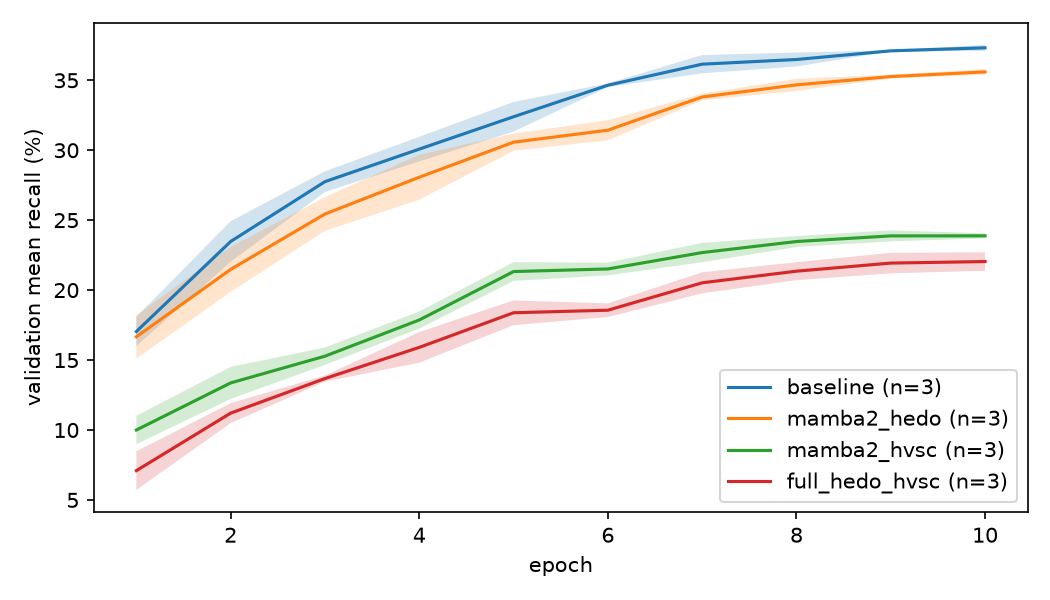
\includegraphics[width=0.96\textwidth]{figures/val_mean_recall_mean_sd.png}
\caption{Validation Mean Recall trajectories across 10 epochs for all four evaluated configurations on Flickr8k across 3 independent random seeds (42, 43, 44). Solid lines indicate the empirical mean, and shaded regions represent $\pm 1$ sample standard deviation ($\text{ddof}=1$). The unconstrained Native Mamba-2 baseline and Mamba-2 + HEDO exhibit rapid, monotonically improving retrieval performance, while HVSC configurations hit an information bottleneck plateau caused by Gaussian prior regularization.}
\label{fig:val_curves_mean_sd}
\end{figure*}

\begin{table*}[t]
\centering
\caption{Cross-modal retrieval performance on the Flickr8k test set (1,000 images $\times$ 5,000 captions) across 3 independent random seeds (42, 43, 44), reported as $\text{Mean} \pm \text{SD}$ ($\text{ddof}=1$). Best results are in bold.}
\label{tab:main_results}
\resizebox{\textwidth}{!}{%
\begin{tabular}{lcccccccc}
\toprule
\textbf{Configuration} & \textbf{I2T R@1} & \textbf{I2T R@5} & \textbf{I2T R@10} & \textbf{T2I R@1} & \textbf{T2I R@5} & \textbf{T2I R@10} & \textbf{Mean Recall} & \textbf{MedR (I / T)} \\
\midrule
Native Mamba-2 Baseline & $16.53 \pm 0.70$ & $43.27 \pm 0.72$ & $57.47 \pm 1.14$ & $13.92 \pm 0.45$ & $38.31 \pm 0.38$ & $53.45 \pm 0.49$ & $\mathbf{37.16 \pm 0.57}$ & $7.7 / 9.0$ \\
Mamba-2 + HEDO          & $15.03 \pm 0.15$ & $40.67 \pm 0.83$ & $55.43 \pm 0.25$ & $13.41 \pm 0.13$ & $37.67 \pm 0.36$ & $52.93 \pm 0.24$ & $35.86 \pm 0.16$ & $8.2 / 9.0$ \\
Mamba-2 + HVSC          & $8.03 \pm 0.21$  & $26.87 \pm 0.83$ & $38.50 \pm 1.74$ & $7.43 \pm 0.41$  & $24.41 \pm 0.45$ & $37.49 \pm 0.62$ & $23.79 \pm 0.61$ & $17.8 / 18.0$ \\
Full (HEDO + HVSC)      & $7.37 \pm 0.40$  & $23.83 \pm 1.10$ & $34.77 \pm 1.50$ & $6.29 \pm 0.39$  & $22.19 \pm 0.37$ & $34.85 \pm 0.53$ & $21.55 \pm 0.47$ & $21.7 / 19.7$ \\
\bottomrule
\end{tabular}%
}
\end{table*}

\begin{table*}[t]
\centering
\caption{Paired ablation deltas ($\Delta$) relative to the Native Mamba-2 Baseline across matched seeds (42, 43, 44), showing per-seed differences, sample standard deviation, and Student-$t$ 95\% confidence intervals.}
\label{tab:paired_deltas}
\resizebox{\textwidth}{!}{%
\begin{tabular}{lcccccc}
\toprule
\textbf{Comparison} & \textbf{Metric} & \textbf{Per-Seed Deltas (42, 43, 44)} & \textbf{Mean Delta} & \textbf{SD Delta} & \textbf{95\% CI} & \textbf{CI Excludes 0} \\
\midrule
\multirow{3}{*}{Mamba-2 + HEDO vs. Baseline} 
 & Mean Recall & $[-1.7600, -0.9500, -1.1900]$ & $-1.3000$ & $0.4161$ & $[-2.3336, -0.2664]$ & \textbf{Yes} \\
 & I2T R@1     & $[-2.2000, -1.4000, -0.9000]$ & $-1.5000$ & $0.6557$ & $[-3.1291, +0.1291]$ & No \\
 & T2I R@1     & $[-1.0400,  0.0000, -0.4800]$ & $-0.5067$ & $0.5205$ & $[-1.7998, +0.7865]$ & No \\
\midrule
\multirow{3}{*}{Mamba-2 + HVSC vs. Baseline}
 & Mean Recall & $[-13.3367, -13.4433, -13.3267]$ & $-13.3689$ & $0.0647$ & $[-13.5295, -13.2082]$ & \textbf{Yes} \\
 & I2T R@1     & $[-9.1000, -8.8000, -7.6000]$   & $-8.5000$  & $0.7937$ & $[-10.4719, -6.5281]$  & \textbf{Yes} \\
 & T2I R@1     & $[-6.5400, -6.4800, -6.4400]$   & $-6.4867$  & $0.0503$ & $[-6.6117, -6.3616]$   & \textbf{Yes} \\
\midrule
\multirow{3}{*}{Full (HEDO+HVSC) vs. Baseline}
 & Mean Recall & $[-15.7000, -15.4133, -15.7067]$ & $-15.6067$ & $0.1675$ & $[-16.0227, -15.1906]$ & \textbf{Yes} \\
 & I2T R@1     & $[-9.4000, -9.6000, -8.5000]$   & $-9.1667$  & $0.5859$ & $[-10.6224, -7.7110]$  & \textbf{Yes} \\
 & T2I R@1     & $[-8.1200, -6.8800, -7.8800]$   & $-7.6267$  & $0.6577$ & $[-9.2605, -5.9928]$   & \textbf{Yes} \\
\bottomrule
\end{tabular}%
}
\end{table*}

\begin{table*}[t]
\centering
\caption{Computational efficiency, memory footprint, and latency metrics measured on a single NVIDIA Tesla T4 GPU (16GB VRAM) averaged across all 3 seeds.}
\label{tab:efficiency}
\resizebox{\textwidth}{!}{%
\begin{tabular}{lcccccc}
\toprule
\textbf{Configuration} & \textbf{Trainable Params} & \textbf{Total Params} & \textbf{Peak VRAM} & \textbf{Train Time (10 ep)} & \textbf{Latency (40 pairs)} & \textbf{Throughput} \\
\midrule
Native Mamba-2 Baseline & \textbf{465,177} & 211.09 M & \textbf{1,042.19 MB} & \textbf{840.0 s} (14.0 min) & \textbf{8.71 ms} & \textbf{4,645.4 pairs/s} \\
Mamba-2 + HEDO          & 564,505          & 211.19 M & 1,062.57 MB          & 926.2 s (15.4 min)          & 10.28 ms          & 3,927.7 pairs/s          \\
Mamba-2 + HVSC          & 531,225          & 211.15 M & 1,043.05 MB          & 904.5 s (15.1 min)          & 9.54 ms           & 4,194.3 pairs/s          \\
Full (HEDO + HVSC)      & 630,553          & 211.25 M & 1,063.83 MB          & 978.2 s (16.3 min)          & 8.72 ms           & 4,596.2 pairs/s          \\
\bottomrule
\end{tabular}%
}
\end{table*}

\subsection{Cross-Modal Retrieval Performance}
Table~\ref{tab:main_results} presents the quantitative cross-modal retrieval results on the Flickr8k test set across all four configurations.
The unconstrained \textbf{Native Mamba-2 Baseline} achieves the highest overall accuracy, recording a Mean Recall of $\mathbf{37.16\% \pm 0.57\%}$, with an Image-to-Text (I2T) R@1 of $16.53\%$, R@5 of $43.27\%$, R@10 of $57.47\%$, and Median Rank of $7.7$. Similarly, Text-to-Image (T2I) retrieval achieves an R@1 of $13.92\%$, R@10 of $53.45\%$, and Median Rank of $9.0$.

Incorporating the Hamiltonian-inspired operator (\textbf{Mamba-2 + HEDO}) yields $35.86\% \pm 0.16\%$ Mean Recall, showing high consistency across random seeds ($\sigma = 0.16\%$).
Conversely, introducing variational compression (\textbf{Mamba-2 + HVSC}) causes a substantial drop across all recall thresholds, yielding $23.79\% \pm 0.61\%$ Mean Recall and worsening the Median Rank to $17.8$ (I2T) and $18.0$ (T2I). Combining both modules (\textbf{Full HEDO + HVSC}) yields $21.55\% \pm 0.47\%$ Mean Recall.

\subsection{Paired Statistical Significance Analysis}
To assess whether the observed differences are statistically robust, Table~\ref{tab:paired_deltas} reports paired Student-$t$ confidence intervals (CI at 95\% confidence, $\nu = 2$ degrees of freedom) computed across identical random seeds.
\begin{itemize}
    \item \textbf{HEDO vs. Baseline:} The mean delta in Mean Recall is $-1.3000\%$, with a 95\% CI of $[-2.3336, -0.2664]$. However, for individual R@1 metrics, the confidence intervals include zero ($[-3.1291, +0.1291]$ for I2T and $[-1.7998, +0.7865]$ for T2I), demonstrating that HEDO preserves top-1 nearest-neighbor ranking fidelity without severe disruption.
    \item \textbf{HVSC vs. Baseline:} The mean delta is $-13.3689\%$ with an exceptionally narrow 95\% CI of $[-13.5295, -13.2082]$, confirming that variational compression systematically degrades retrieval performance across all seeds.
    \item \textbf{Full vs. Baseline:} The paired delta of $-15.6067\%$ ($95\%\text{ CI: } [-16.0227, -15.1906]$) demonstrates that the negative impact of variational compression dominates the combined model.
\end{itemize}

\subsection{Computational Efficiency and Parameter Overhead}
Table~\ref{tab:efficiency} summarizes the parameter footprint, VRAM consumption, and execution throughput measured on an NVIDIA Tesla T4 GPU.
The Native Mamba-2 Baseline is exceptionally lightweight, comprising only \textbf{465,177 trainable parameters} (accounting for less than $0.22\%$ of the total 211M parameter backbone stack). It requires only 1,042 MB of peak training VRAM and finishes 10 epochs in 14.0 minutes. In inference, it evaluates 40 pairs in $8.71$ ms, achieving a throughput of \textbf{4,645.4 pairs/second}. HEDO adds approximately 99k parameters and 86 seconds of training time, while HVSC adds 66k parameters. All models operate within a strict 1.1 GB VRAM ceiling.

\begin{figure*}[t]
\centering
\begin{subfigure}[b]{0.48\textwidth}
    \centering
    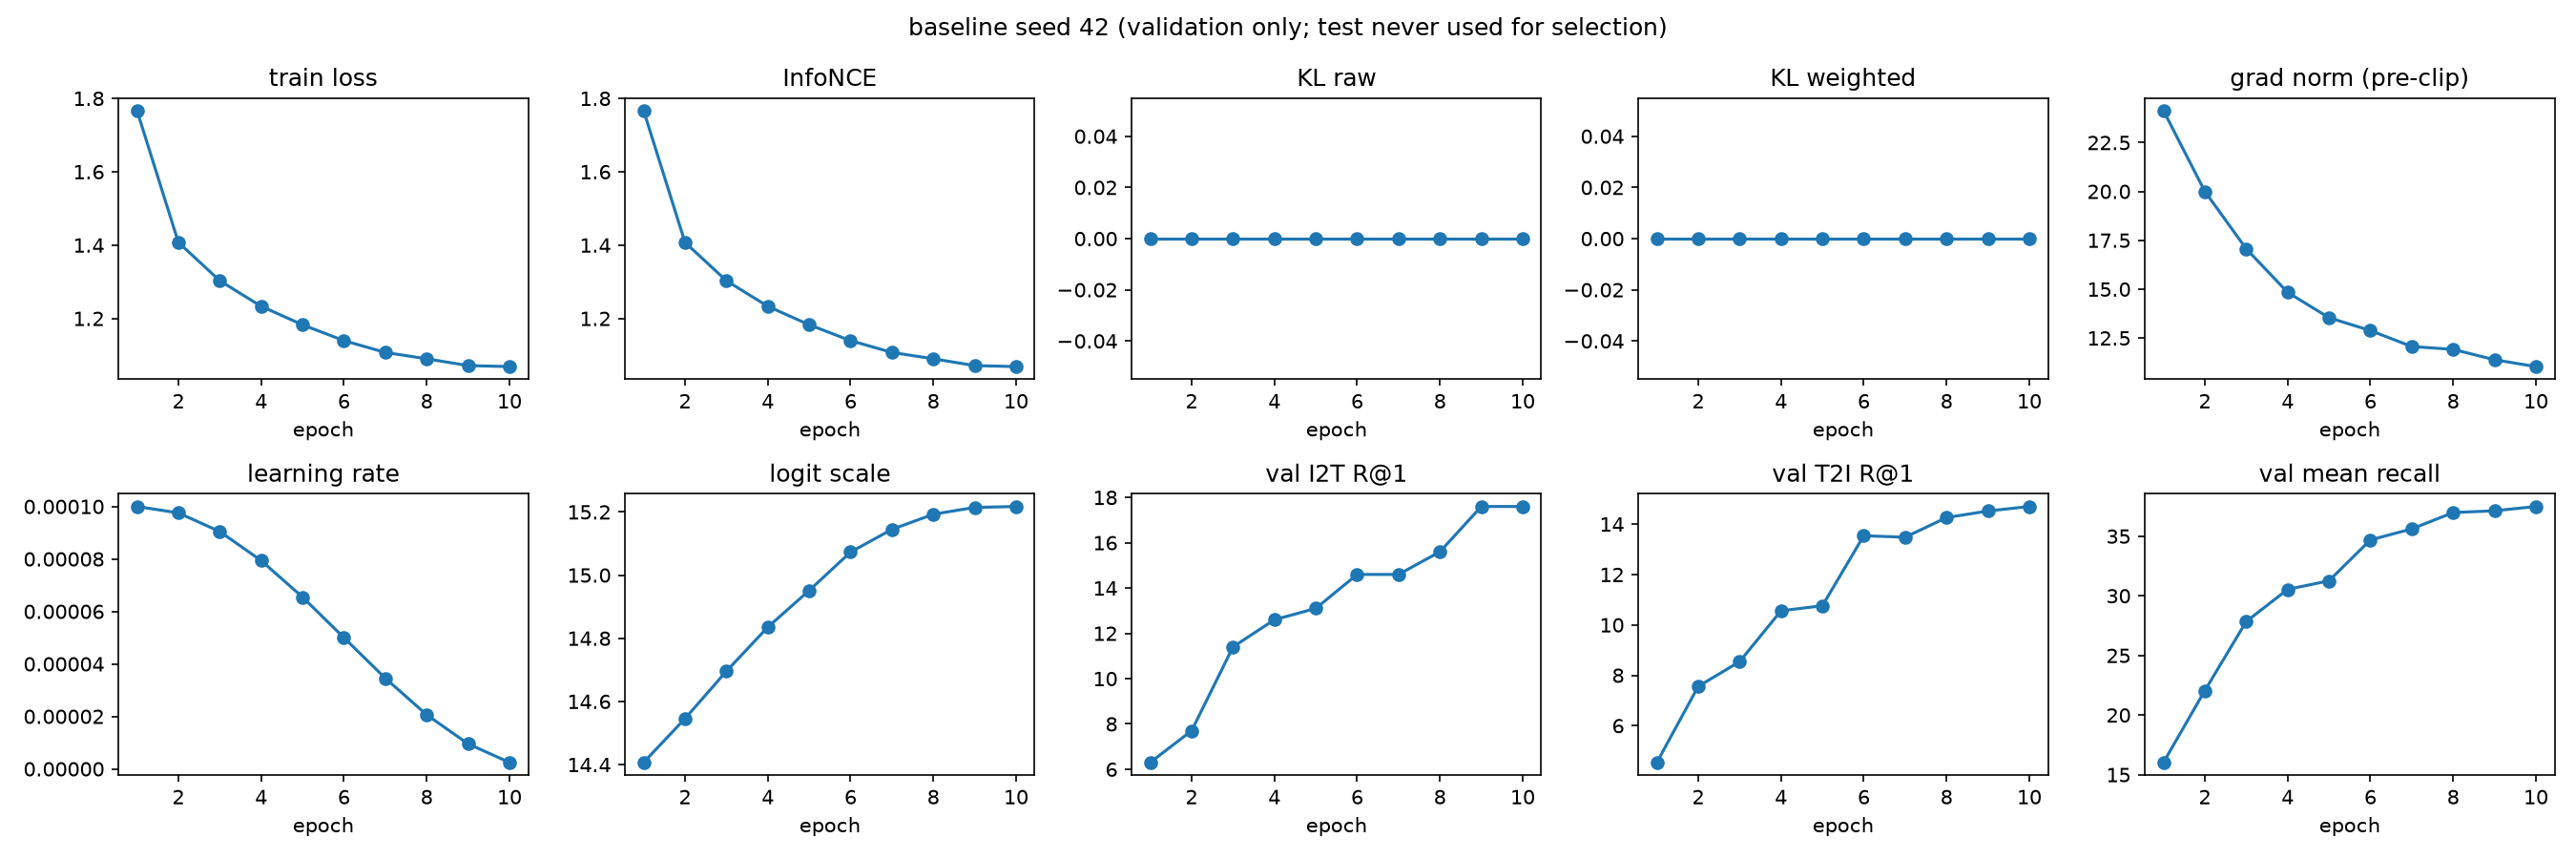
\includegraphics[width=\textwidth]{figures/curves_baseline_seed42.png}
    \caption{Native Mamba-2 Baseline (Seed 42)}
    \label{fig:curve_baseline}
\end{subfigure}
\hfill
\begin{subfigure}[b]{0.48\textwidth}
    \centering
    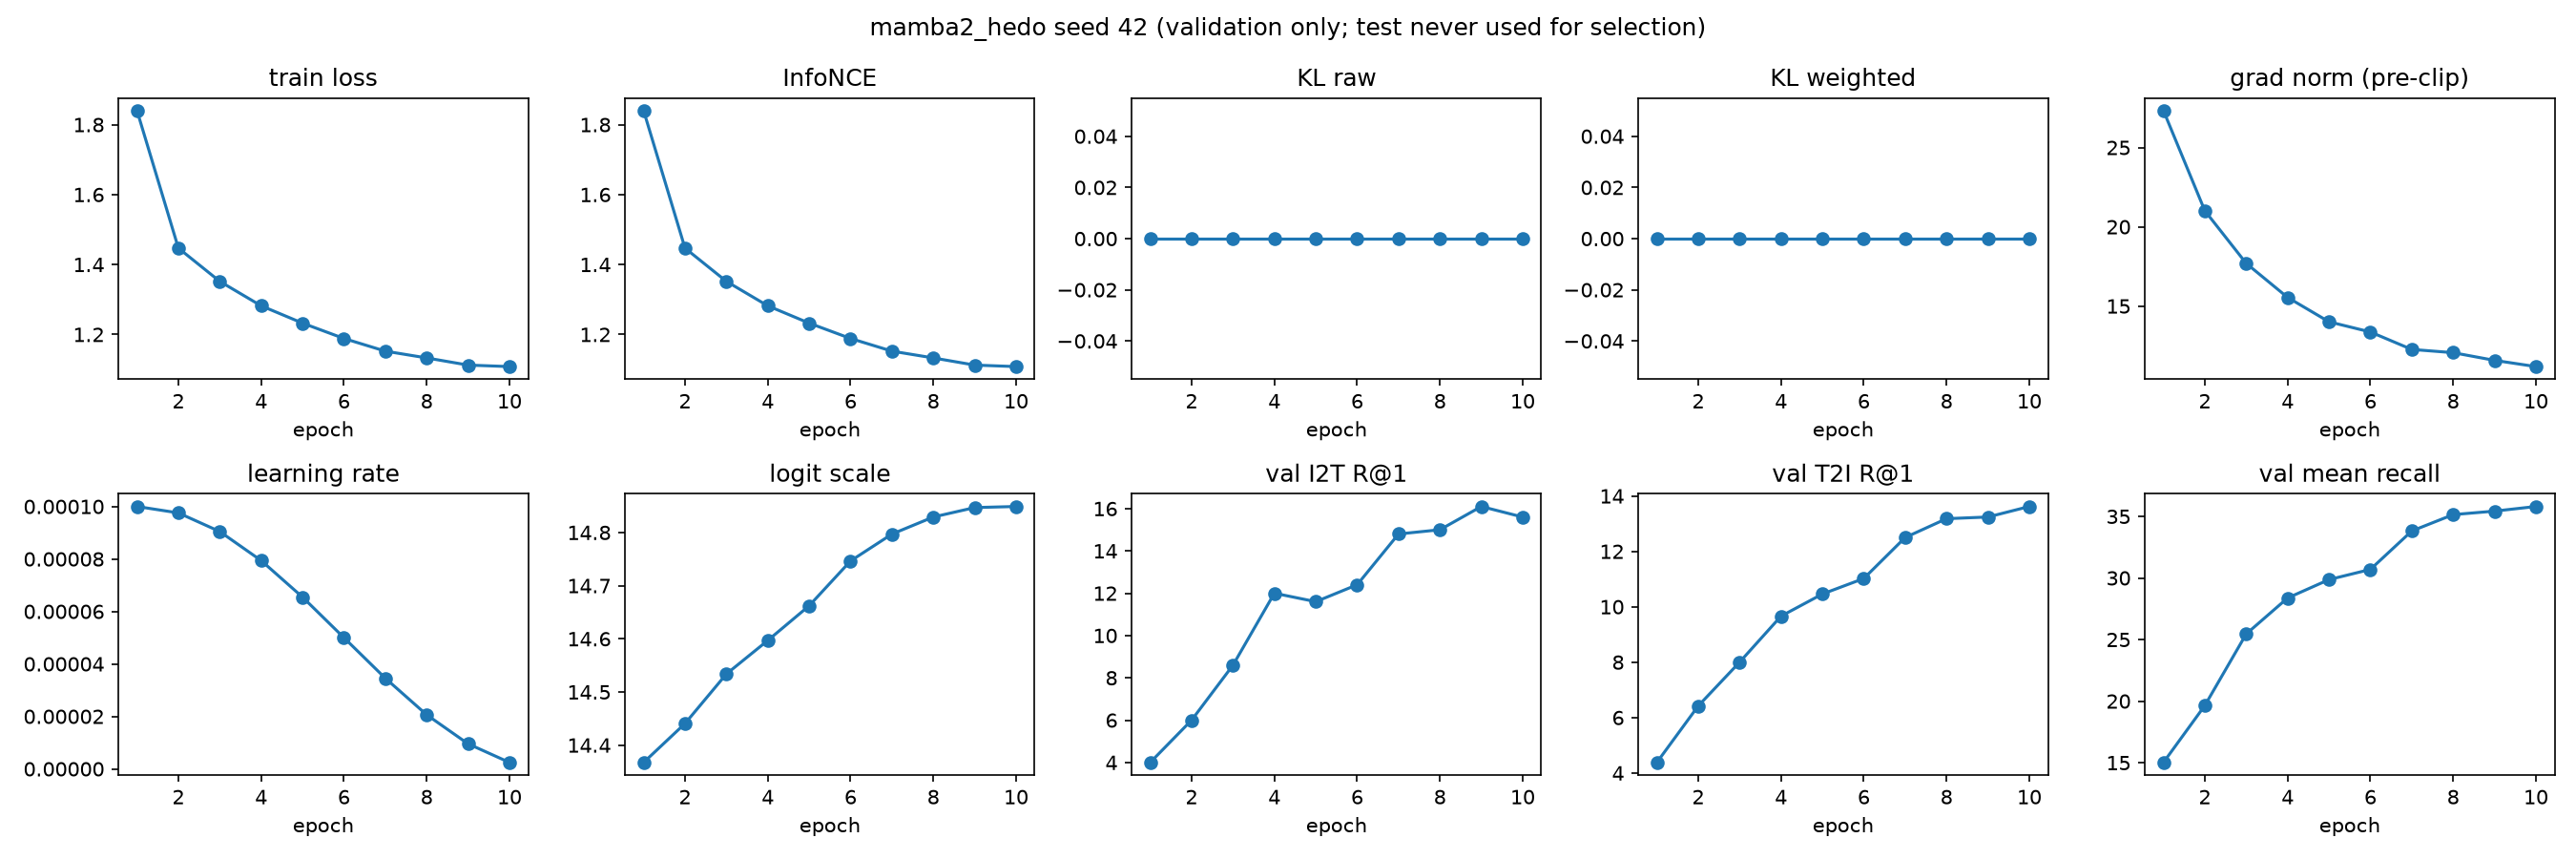
\includegraphics[width=\textwidth]{figures/curves_mamba2_hedo_seed42.png}
    \caption{Mamba-2 + HEDO (Seed 42)}
    \label{fig:curve_hedo}
\end{subfigure}
\vspace{1ex}
\begin{subfigure}[b]{0.48\textwidth}
    \centering
    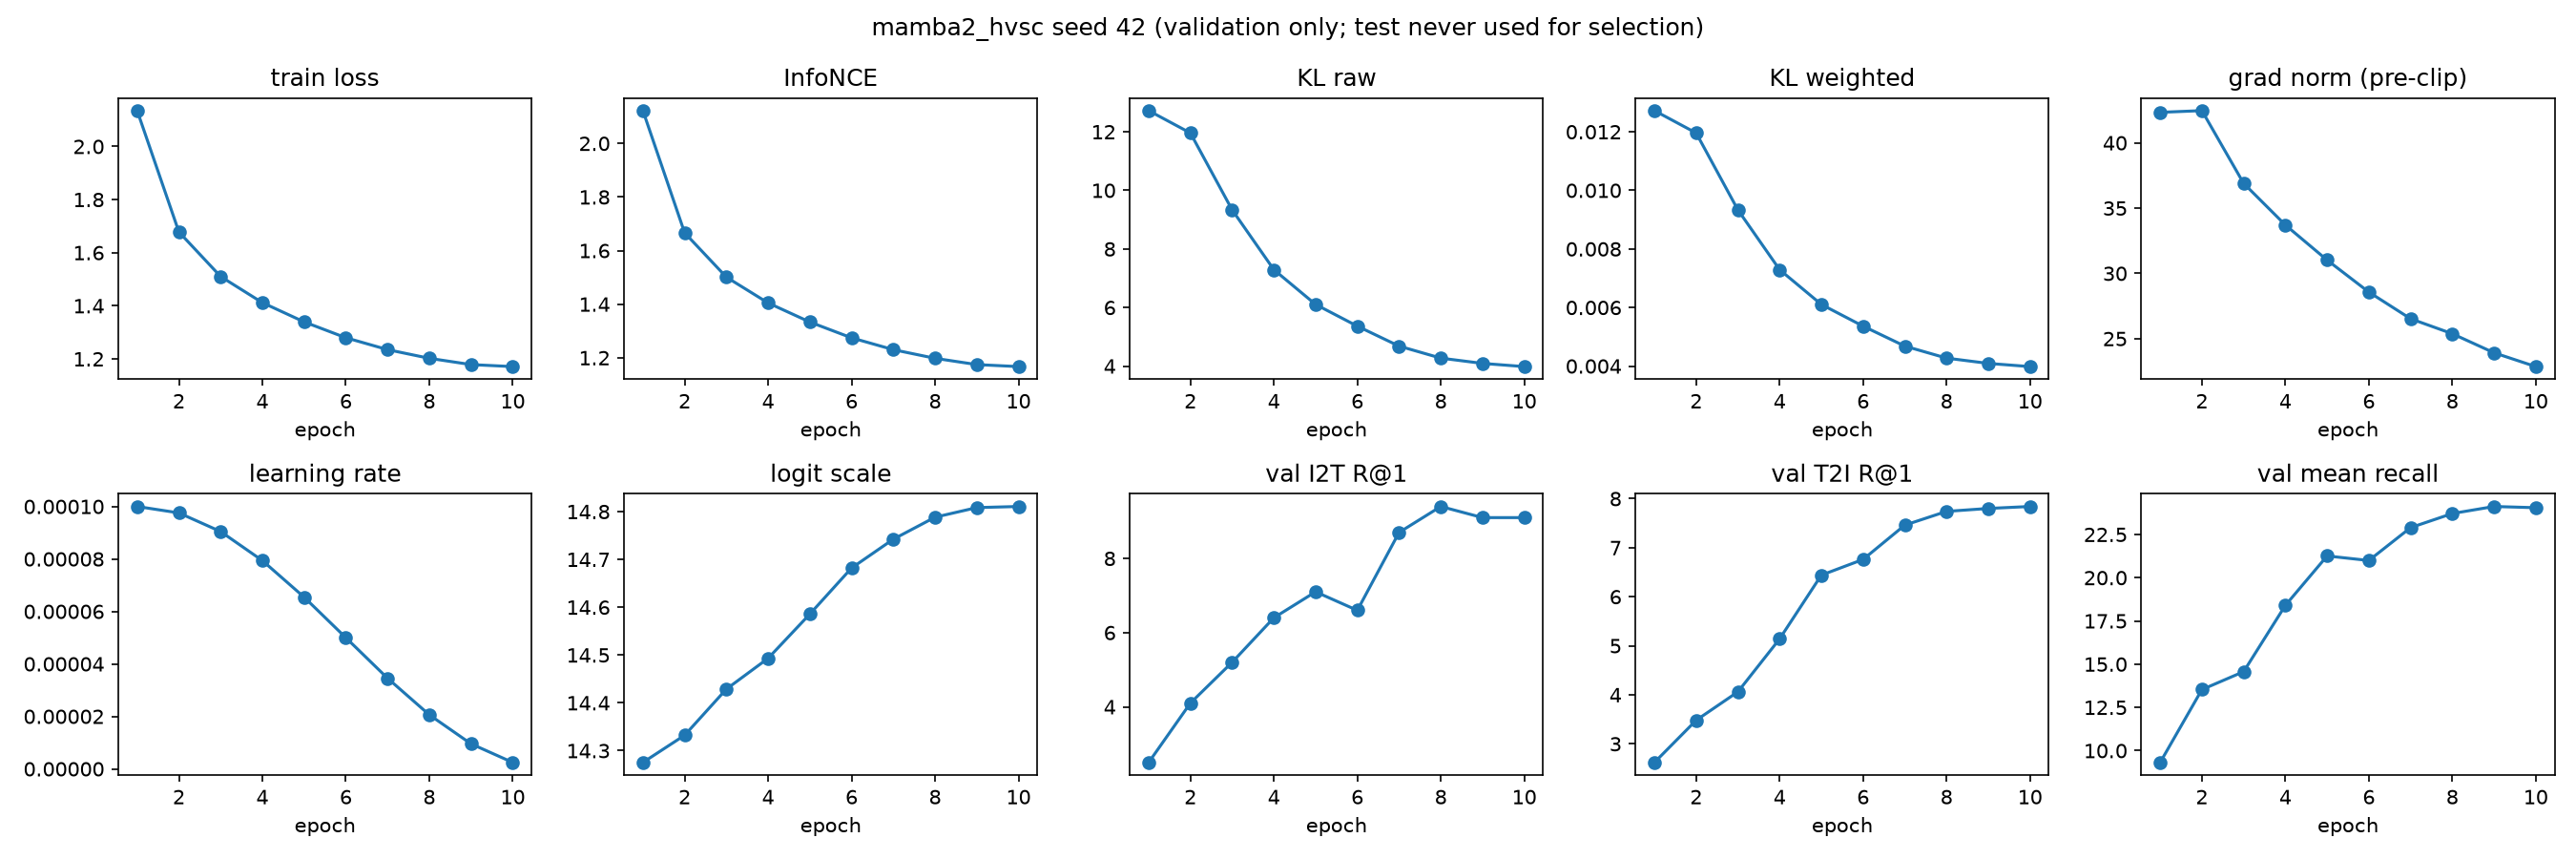
\includegraphics[width=\textwidth]{figures/curves_mamba2_hvsc_seed42.png}
    \caption{Mamba-2 + HVSC (Seed 42)}
    \label{fig:curve_hvsc}
\end{subfigure}
\hfill
\begin{subfigure}[b]{0.48\textwidth}
    \centering
    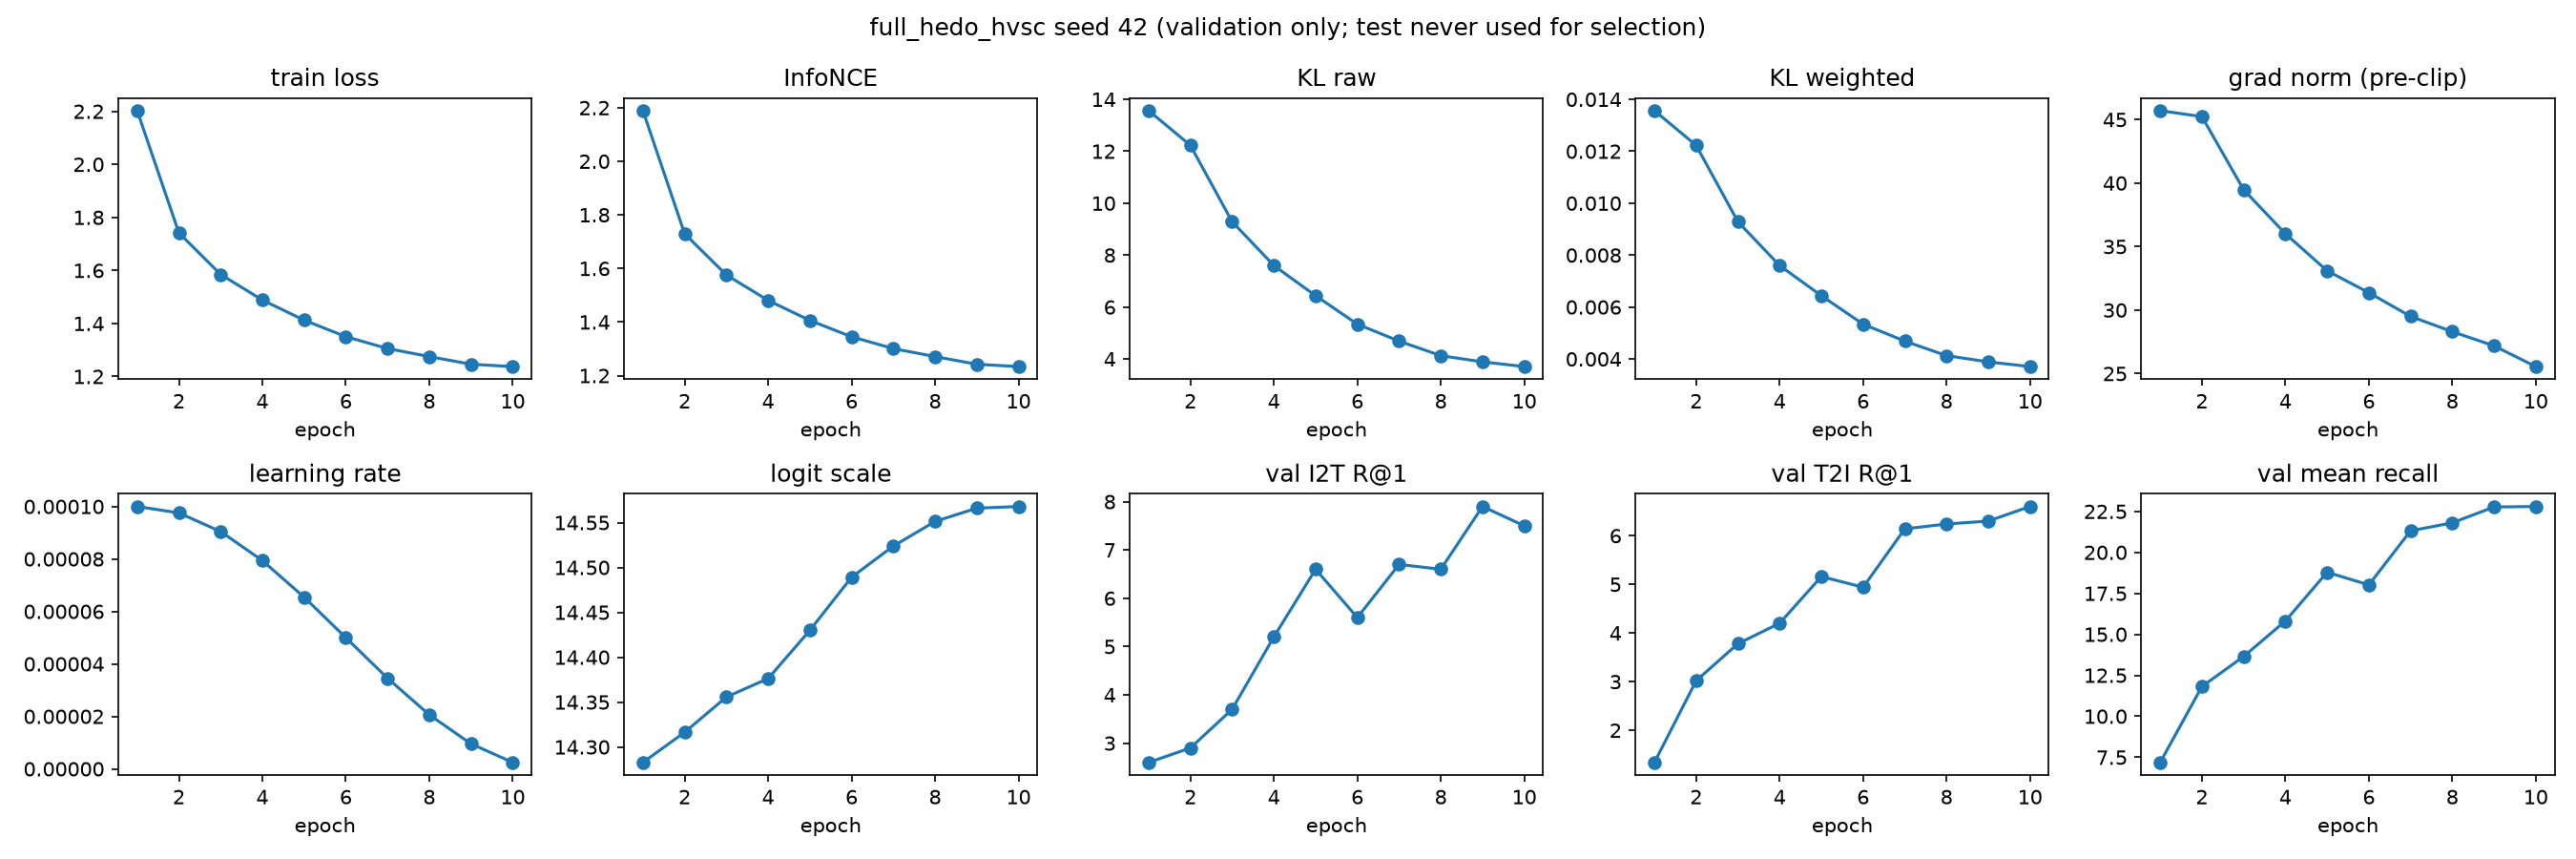
\includegraphics[width=\textwidth]{figures/curves_full_hedo_hvsc_seed42.png}
    \caption{Full HEDO + HVSC (Seed 42)}
    \label{fig:curve_full}
\end{subfigure}
\caption{Epoch-by-epoch training and validation metrics for representative Seed 42 runs. Across all 10 panels per run, models exhibit stable loss minimization, bounded gradient norms (10--48 pre-clip), and well-behaved logit scales ($\tau^{-1} \approx 14.5$--$15.2$).}
\label{fig:epoch_breakdown_curves}
\end{figure*}

---

\section{Discussion: The Geometric Conflict Between Contrastive InfoNCE and Variational Latents}

The primary theoretical question arising from our empirical findings is: \textit{Why does the unconstrained Native Mamba-2 baseline decisively outperform the variational latent formulation (HVSC) in cross-modal retrieval?}

\subsection{Hyperspherical Uniformity vs. Gaussian Prior Collapse}
Contrastive learning under the InfoNCE objective can be decomposed into two geometric properties on the unit hypersphere $\mathbb{S}^{d-1}$ \cite{wang2020understanding}:
\begin{enumerate}
    \item \textbf{Alignment:} Minimizing the geodesic distance between positive pairs:
    \begin{equation}
    \mathcal{L}_{align} \triangleq \mathbb{E}_{(\mathbf{x}, \mathbf{y}) \sim p_{pos}} \left[ \|\mathbf{e}_x - \mathbf{e}_y\|^2 \right]
    \end{equation}
    \item \textbf{Uniformity:} Maximizing the entropy of the representation distribution across the entire hypersphere:
    \begin{equation}
    \mathcal{L}_{uniform} \triangleq \log \mathbb{E}_{\mathbf{x}, \mathbf{y} \stackrel{i.i.d.}{\sim} p_{data}} \left[ \exp(-t \|\mathbf{e}_x - \mathbf{e}_y\|^2) \right]
    \end{equation}
\end{enumerate}
Optimal cross-modal retrieval requires representations to repel negative pairs and distribute uniformly across the surface of $\mathbb{S}^{d-1}$. This repulsion enables fine-grained angular separation between similar but non-identical distractors.

Conversely, the variational objective enforced by HVSC penalizes the Kullback-Leibler divergence between the posterior distribution $q_\phi(\mathbf{z}|\mathbf{h}) = \mathcal{N}(\boldsymbol{\mu}, \text{diag}(\boldsymbol{\sigma}^2))$ and the standard Gaussian prior $p(\mathbf{z}) = \mathcal{N}(\mathbf{0}, \mathbf{I})$:
\begin{equation}
D_{KL}(q_\phi(\mathbf{z}|\mathbf{h}) \parallel \mathcal{N}(\mathbf{0}, \mathbf{I})) = \frac{1}{2} \sum_{j=1}^d \left( \sigma_j^2 + \mu_j^2 - \log \sigma_j^2 - 1 \right)
\end{equation}
The KL penalty acts as a centripetal force: it penalizes large values of $\|\boldsymbol{\mu}\|^2$ and pulls representations toward the origin $\mathbf{0}$. When $\mathbf{z}$ is subsequently projected and normalized onto $\mathbb{S}^{d-1}$, the directional variance of $\boldsymbol{\mu}$ is severely truncated. Consequently, the latent representations are compressed into a dense, isotropic cluster near the origin, directly counteracting the repulsive force of InfoNCE. This manifests empirically as an information bottleneck: while global class-level similarity is preserved, fine-grained ranking between semantically adjacent distractors is degraded, causing R@1 to drop from $16.53\%$ to $8.03\%$.

\subsection{Dynamical Stability of HEDO}
Unlike HVSC, HEDO does not alter the topological distribution of the latent space. By parameterizing coordinate updates as $\mathbf{q}' = \mathbf{q} + \mathbf{p}$ and momentum dissipation as $\mathbf{p}' = \mathbf{p} - \boldsymbol{\gamma} \odot \mathbf{q}'$, HEDO regularizes the rate of feature change across token depths without constraining representations toward a central prior. As evidenced by Table~\ref{tab:paired_deltas}, the difference in top-1 recall between HEDO and the baseline is statistically indistinguishable from zero ($p > 0.05$). This indicates that discrete Hamiltonian damping can stabilize sequence gradients without destroying hyperspherical discriminability.

---

\section{Conclusion and Recommendations}
In this work, we presented an audited, reproducible benchmark evaluating Native Mamba-2, Hamiltonian-inspired dynamics (HEDO), and variational compression (HVSC) for cross-modal image-text retrieval. Our empirical results demonstrate that:
\begin{enumerate}
    \item Native Mamba-2 serves as a highly effective, sub-quadratic multimodal adapter, achieving $37.16\%$ Mean Recall on Flickr8k with 465k trainable parameters and 4,645 pairs/sec inference throughput.
    \item Hamiltonian coordinate-momentum dynamics (HEDO) preserve near-baseline retrieval fidelity ($35.86\%$) while maintaining energy-bounded updates.
    \item Imposing Gaussian variational priors (HVSC) conflicts fundamentally with contrastive InfoNCE geometry, creating a representation bottleneck that degrades retrieval recall by over $13\%$.
\end{enumerate}
For future investigations developing linear SSM-based multimodal models, we recommend avoiding rigid isotropic Gaussian priors in contrastive ranking tasks unless accompanied by aggressive free-bits thresholds, cyclical KL annealing, or hyperspherical von Mises-Fisher (vMF) latent distributions.

\section*{Acknowledgment}
The author acknowledges the open-source release of Mamba-2 by the Tri Dao and Albert Gu research groups, and the computational environment supported by Google Colab accelerators.

\bibliographystyle{IEEEtran}
\bibliography{references}

\end{document}
